% \section{Seperation of Frontend and Backend}


\subsection{Evolution}
With the increasing complexity of a web app and high demand of agile development, people are always thinking about how to improve patterns of the workflow in web development as well as the architecture of a web app. To achieve better scalability, maintainability and ubiquity of a web app, the architecture of an entire web app has been envolving in the past several years .

\subsubsection{Early Age}
At the early age of web development, the backend did all jobs for both client side(browser) and server side, such as rendering, calling system service, composing data, etc. Figure \ref{fig:3.1} shows the overview of web architecture:
\begin{figure}[!htbp]
  \centering
    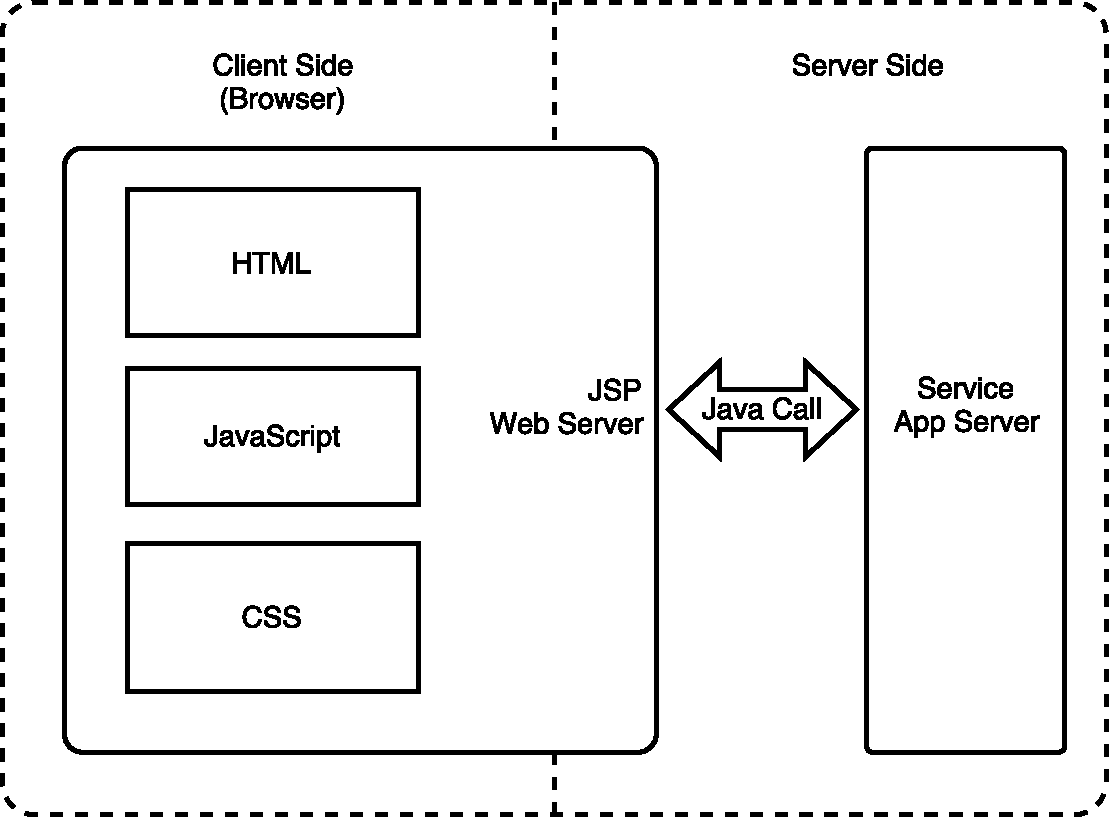
\includegraphics[width=0.8\textwidth]{Figures/tech-web-arch-early.pdf}
  \caption{Web architecture in early age}
  \label{fig:3.1}
\end{figure}
The advantage of this pattern is clear: The development and deployment are simple and straightforward, if the bussiness logic doesn't become complexer. But with the increasing complexity of the product, the problems shows up:
\begin{enumerate}
\item
Development of frontend heavily depends on the whore development environment. Developers have to start up all the tools and services for testing and debugging only some small changes on view. In most cases, the frontend developer who isn't familar with the backend needs help while intergrating the new views into the system. Not only the efficiency of development, but also the cost of communication between frontend developer and backend developer are huge problems.
\item
The own responsibility of front-end and back-end mess up, which could be expressed by the commingled codes from different layers, for example there is no clear boundry from data processing tp data representing. The maintainability of the project becomes worse and worse with the increasing complexity.
\end{enumerate}

It's really significant to improve the maintainability of code, as well as the efficiency and resrationality of division of work from both front-end and back-end in the whole web development phase. In the section below, a evolution of the technical architecture will reveal how these problems are solved.

\subsubsection{Web 2.0}
Along with the birth of Gmail\footnote{https://mail.google.com/} in 2004, which is noted for its pioneering use of \gls{Ajax}, the web application started to behave more interactively. Browser began to take over the job of data fetching, processing, rendering, such a sequence of workflow which could only be done by the server side formerly.

The architecture in Web 2.0 generation is presented in figure \ref{fig:3.2}.

\begin{figure}[!htbp]
  \centering
    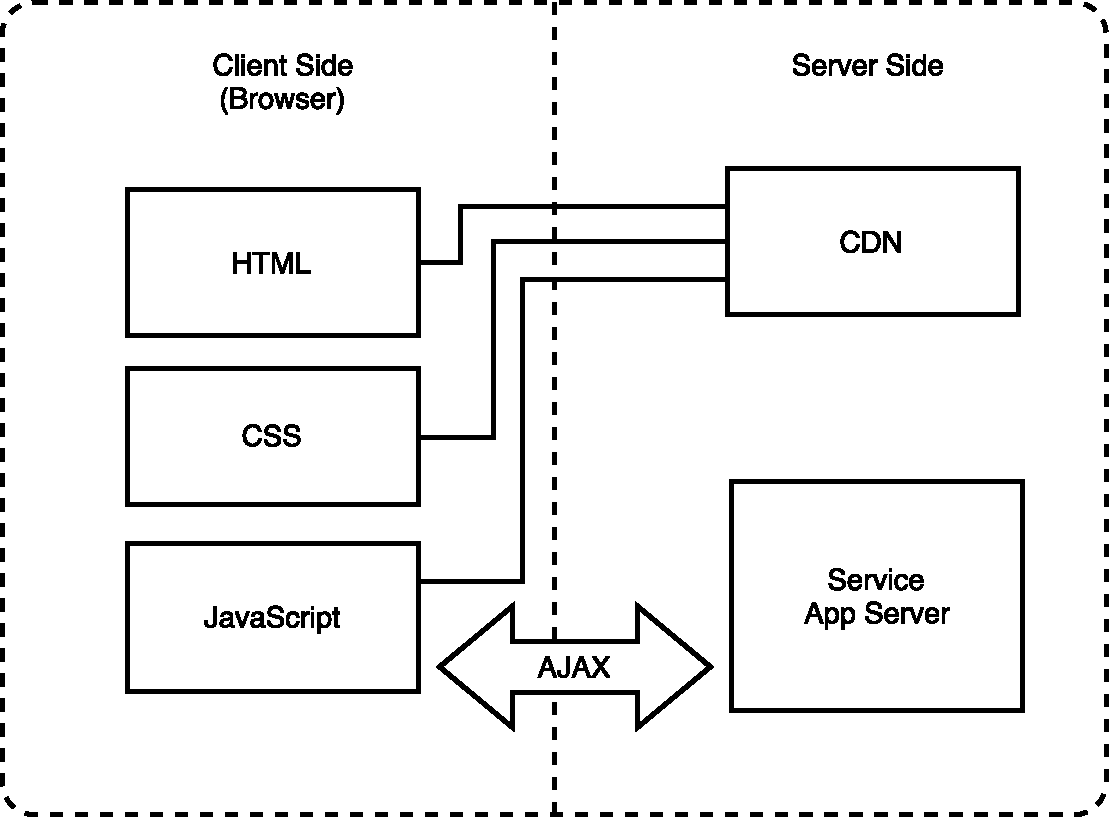
\includegraphics[width=0.8\textwidth]{Figures/tech-web-arch-2.pdf}
  \caption{Web 2.0 architecture}
  \label{fig:3.2}
\end{figure}

By using Ajax, the client has the ability to fetching data stream asynchronously, after which the client will consume the data and render it into the specific section of view. Usability was dramatically improved, because the entired view represented to users will not be refreshed and the front-end is able to process and render data in its own intension, which means more flexible control of the consumption of data.

\subsubsection{Single Page App}

With the evolution of web technologies and promotion of these technologies in modern browswers by brower vendors, a new web development model called \gls{SPA} was proposed and caught the developers' eye. The back-end is no more responsible for rendering and view controling, it only take charge of providing services for the front-end.

\begin{figure}[!htbp]
  \centering
    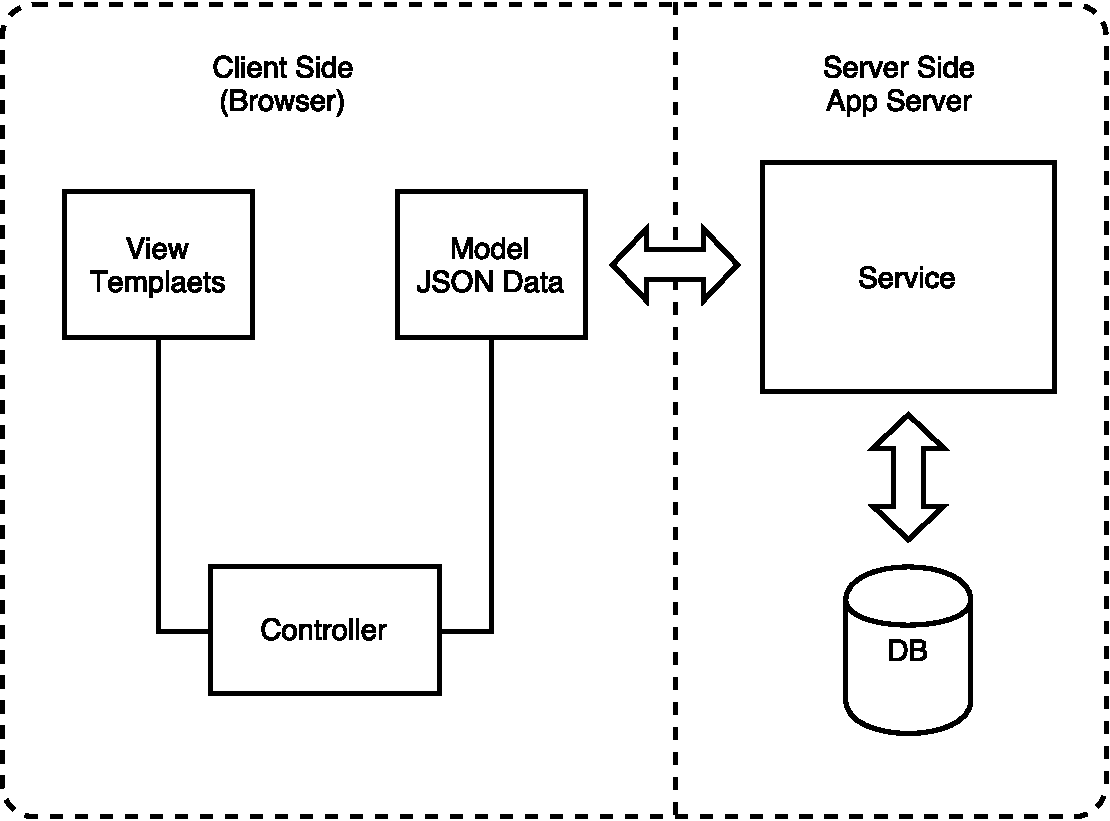
\includegraphics[width=0.8\textwidth]{Figures/tech-web-arch-spa.pdf}
  \caption{SPA architecture}
  \label{fig:3.3}
\end{figure}

The structure in figure \ref{fig:3.3} shows that the client side has the full control of view rendering and data consumption after data acquisition through web services which is released by back-end with promised protocol. All rendering tasks was stripped off from the server side, which means that the server side achieves more efficiency and concentrate more on the core bussiness logics.

But more responsibility in front-end means more complexity. How to reduce the complexity and increace the maintainability of a front-end project becomes a significant problem. Developers come up with an new envolved variant of SPA as demonstrated in figure \ref{fig:3.4}.

\begin{figure}[!htbp]
  \centering
    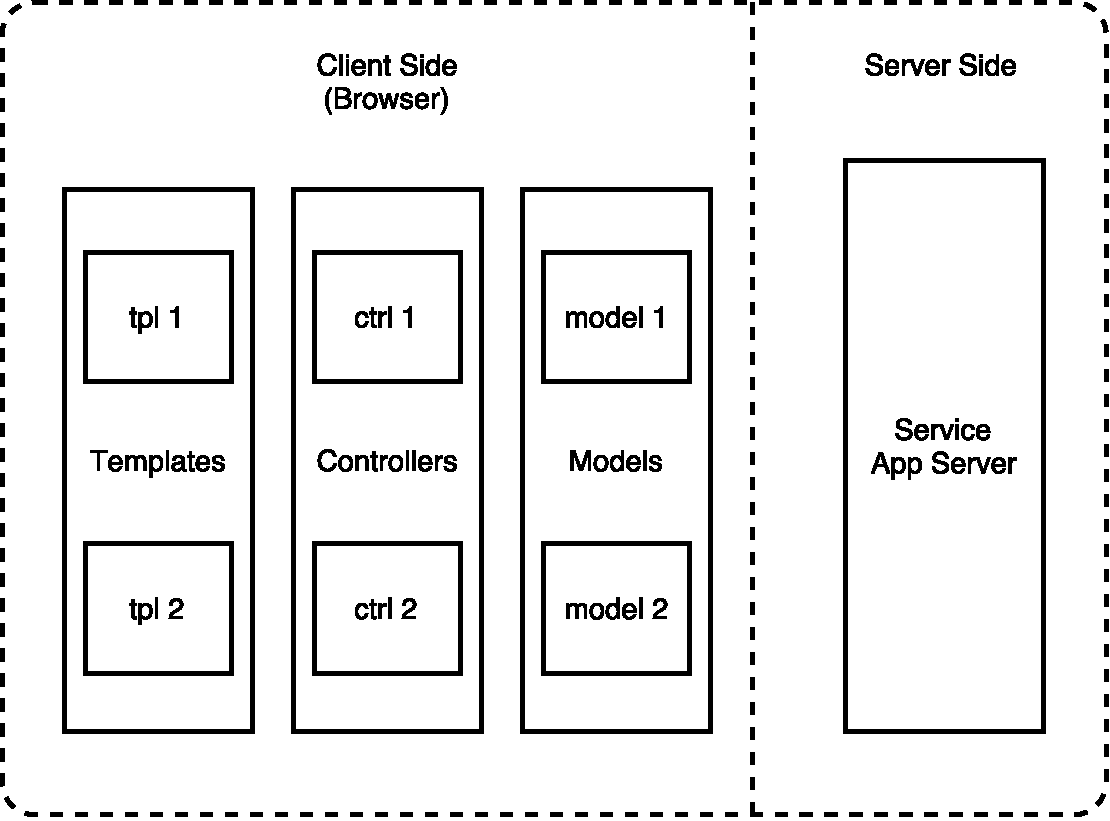
\includegraphics[width=0.8\textwidth]{Figures/tech-web-arch-cmp.pdf}
  \caption{Components in SPA}
  \label{fig:3.4}
\end{figure}

In general, the architecture is componentized and layered into template, controller and model. Each component is isolated and has its own view as well as correlated logics. Front-end frameworks like EmberJS, AngularJS, ReactJS are providing such a approach and development pattern for developers to build modern web apps. With this approach, a giant and complex front-end app is broken up into fine grained components, therefore, components are easy to reuse if the components are well abstrated in a proper way. In addition, the maintaince of each component is also effortless.


\subsubsection{Trade-off}
In summarize, a single-page app has a lot of benefits:
\begin{enumerate}
\item
\textbf{Rational seperation of works from front-end and back-end}: client takes charge of view rendering and data representation, as well as slight data processing if needed; the server focus on providing services of the core logics, persistance of data, and also computational tasks.
\item
\textbf{High interactivity and user experience in client side}: asynchronous data fetching and view rendering implies no more need of hard reloading the page which user is viewing and the current states of the page could also be preserved.
\item
\textbf{Efficiency in server side}: rendering tasks are stripped off from server side.
\item
\textbf{Ubiquity}: with the seperation of services provided by server side, not only the web browser but also other clients in other platforms such as Android, iOS apps are able to access and comsume the services.
\end{enumerate}

But SPA also has its deficiencies:

\begin{enumerate}
\item
\textbf{\gls{SEO} unfriendly}: because the page are not directly rendered by server side, and the web crawlers are not able to run JavaScript codes like a browser does, the site could not be crawled properly under normal circumstances. So if SEO results really matter for the app, SPA is obviously not the best choice.
\item
\textbf{Excessive http connections}: all the data is acquired from different services through diverse \gls{API}s, thus multiple HTTP connections are established and performed parallelly, whose initial time of connections for partial data could be much more than a single connection in the traditional way. So it's highly needed to merge the services and find a balance between data model complexity and time consumption.
\end{enumerate}


\subsection{RESTful Web Service}
REST stands for REpresentational State Transfer. More than a decade after it was introduced, REST has become one of the most essential technologies for Web applications\cite{richardson2008restful}. REST is web standards based architecture which uses HTTP Protocol for data communication. It  centers upon resource  and a resource is accessed by a uniform interface using HTTP standard methods.

In REST architecture, a REST Server simply provides access as well as operations of resources, while a  REST client accesses and manipulates the resources by using different methods. Here URIs are used to locate the resources.


The key principles, which make RESTful applications to be lean and fast, are listed as follows\cite{hamad2010performance}.

\begin{itemize}
  \item \textbf{URI as identifier for resource}:  Through a RESTful web service, clients interact with the targets of the resources exposed. URIs are used as the identifier for resources, which provide a global addressing space for resource requesting and acquisition. 

  \item \textbf{Uniform interface}:  A fixed set of four create, read, update, delete operations is used for manipulation of resources, which could also be represented by HTTP standard methods: PUT, GET, POST, and DELETE.  Retrieving the current state of a resource could be achieved by GET. PUT is for creating a new resource, which can be removed by using DELETE. A new state onto a resource is transferred if POST is used.

  \item \textbf{Self-descriptive messages}:  Resources are decoupled from their representation. As a result, the content of the resource can be accessed in a variety of formats, such as HTML, plain text, JSON, and others.

  \item \textbf{Stateful interactions through hyperlinks}:  Every interaction with a resource is stateless. However, several techniques are able to be applied to achieve the exchange of state, such as URI rewriting, cookies, and hidden form fields. State can be embedded in response messages to point to valid future states of the interaction\cite{tutorial6oracle}. 


\end{itemize}



% \subsection{Continuous Integration}



% \subsection{Operating-system-level virtualization}
